\documentclass{article}
\usepackage[utf8]{inputenc}
\usepackage[T1]{fontenc}
\usepackage[francais]{babel}
\usepackage{minted}
\usepackage{uqac}

%<----------->Meta-Data<----------->

\title{Premier Travail}
\author{Tristan MOLIN\\Florian FICHANT\\Martin LOCQUEVILLE}
\codep{}
\discipline{8INF914 - Visualisation Analytique}
\projet{Etude des algorithmes de dessin d'arbres \\ Travail de session \\ Rapport}
\date{\today}

%<--------------------------------->

\begin{document}

\maketitle

\tableofcontents

\newpage

\mainmatter

\section{Introduction}

L'objectif de notre projet est de parvenir à implémenter en \emph{Python}, au sein de l'outil d'étude de graphe \emph{Tulip}, un algorithme de dessin d'arbre, le plus optimal possible. Pour ce faire, nous avons recueilli et analysé les travaux de recherche dans quatre articles.

Ces articles avaient également comme problématique l'optimisation de dessin de graphe. Chacun d'eux cherchant à optimiser l'implémentation d'un algorithme de dessin d'arbre en prenant en compte les travaux de leurs prédécesseurs (Nous avons pris soin de noter les références de ces articles en fin de rapport).

Suite à l'étude de ces articles, nous allons premièrement implémenter les algorithmes résultant des travaux des auteurs de nos quatre articles de référence. C'est après cela que nous allons écrire de manière optimisée et implémenter notre solution algorithmique en \emph{Python}, en utilisant la bibliothèque \emph{Tulip}.

Pour finir, nous allons étudier plus en détail nos algorithmes à l'aide de jeux de données, permettant de voir ainsi s'ils répondent bien à leur objectif, s'ils peuvent éventuellement être améliorés au niveau du temps d'exécution, de l'écriture du code, etc.


\newpage
\section{Étude préliminaire des articles}

Ayant relevé une continuité Chronologique, dans la mesure où les auteurs reprennent les travaux des précédents articles. Notre étude des articles gardera cet ordre Chronologique.

Avant d'entrer dans l'étude des algorithmes, il est important de définir les caractéristiques principales de ces graphes. Un arbre, tel que défini dans notre premier article \cite{artcile79}, est un graphe plan dans lequel aucune arrête ne se croise, chaque n\oe{}ud du graphe comprend un unique prédécesseur (à l'exception du n\oe{}ud racine: \emph{Root}), un n\oe{}ud en peut se trouver plus proche du \emph{Root} que ses n\oe{}uds parents, le dernier n\oe{}ud d'une branche (n\oe{}ud qui n'a pas de fils) est appellé feuille. La dernière caractéristique de base d'un arbre est l'alignement de ses n\oe{}uds, les n\oe{}uds d’une même hauteur doivent être sur la même ligne de sorte que toutes les hauteurs soient sur des lignes parallèles (cette dernière propriété est noté dans l'article \cite{article79}: \emph{Esthétique 1}).

Maintenant que notre arbre de base est défini, nous pouvons nous intéresser aux problématiques des articles concernant l'implémentation d'algorithme (voir ci-dessous nos propriétés de bases appliquées à un arbre).

\vfill
\begin{figure}[h]
		\begin{center}
			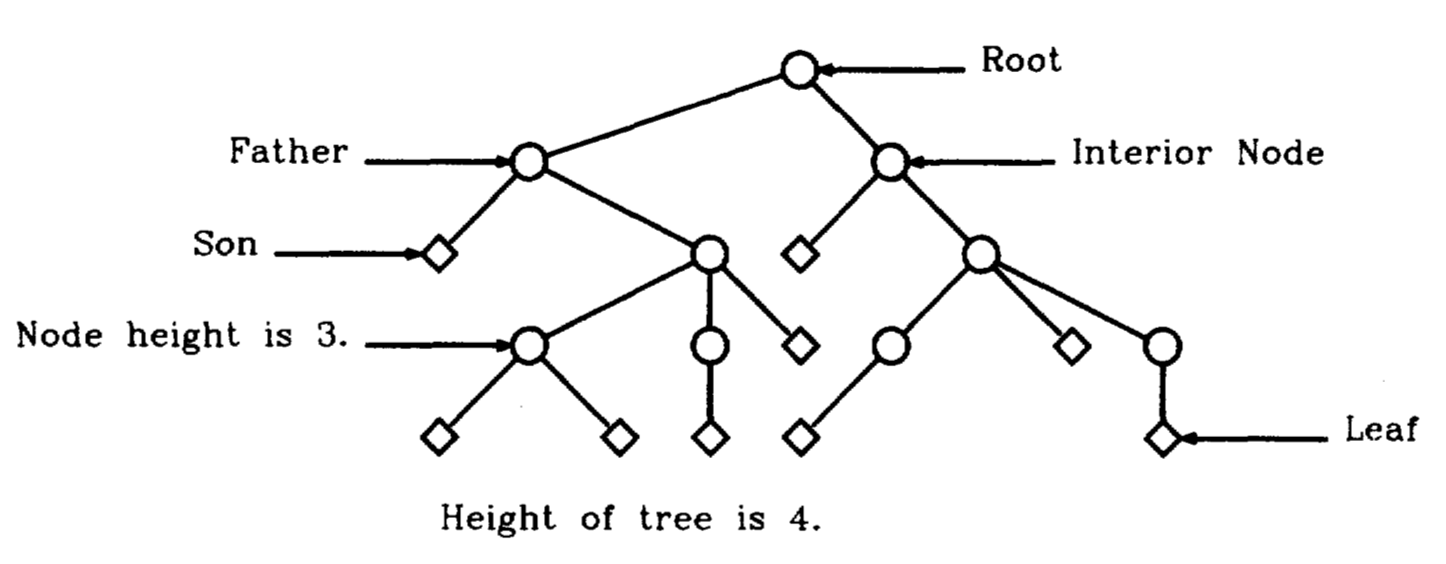
\includegraphics[scale=0.4]{arbre.png}
		\end{center}
	\caption{Exemple d'un arbre d'après nos premières propriétés. \cite{article79}}
  \label{fig:arbre}
\end{figure}
\vfill

\newpage
  \subsection{\emph{Tidy Drawings of Trees}}

  Les auteurs de l'article se sont penchés sur l'optimisation de dessin d'arbre. Dans un soucis d'espace sur lequel représenter les graphe, ils ont posé la problématique suivante (\emph{Limite Physique 1}):  la largeur de l’arbre doit être la plus petite possible (la hauteur est fixée par l’arbre). Pour rappel, la hauteur d'un n\oe{}ud correspond au nombre de branche entre lui et le \emph{Root} (cf: Figure \ref{fig:arbre} page \pageref{fig:arbre}).
    \subsubsection{A Naive Tree Drawer}

    Le premier algorithme (\emph{Algorithme 1}) de dessin d'arbre décri par cet article est \emph{l'algorithme d'arbre naïf}. Il a comme objectif de repondre à la \emph{Limite Physique 1} en optimisant l'espace du graphe.

    Il prend en entrée un arbre, tel que nous l'avons défini plus haut, ainsi que la hauteur de cette arbre et retourne en sortie le même arbre dans lequel la position des n\oe{}uds a changée pour faire en sorte que l'arbre ai la largeur la plus étroite possible.

    Le fonctionnement de cet algorithme comprend une variable qui compte la prochaine coordonnée en $x$ de libre, pour y placer le prochain n\oe{}ud. Pour ce qui est de la coordonnée en $y$ elle correspond à la hauteur du n\oe{}ud dans l'arbre qui a été donnée en paramètre d'entrée de l'algorithme, de cette manière, on respecte toujours l'\emph{Esthétique 1}.

    \vfill
    \begin{figure}[h]
    		\begin{center}
    			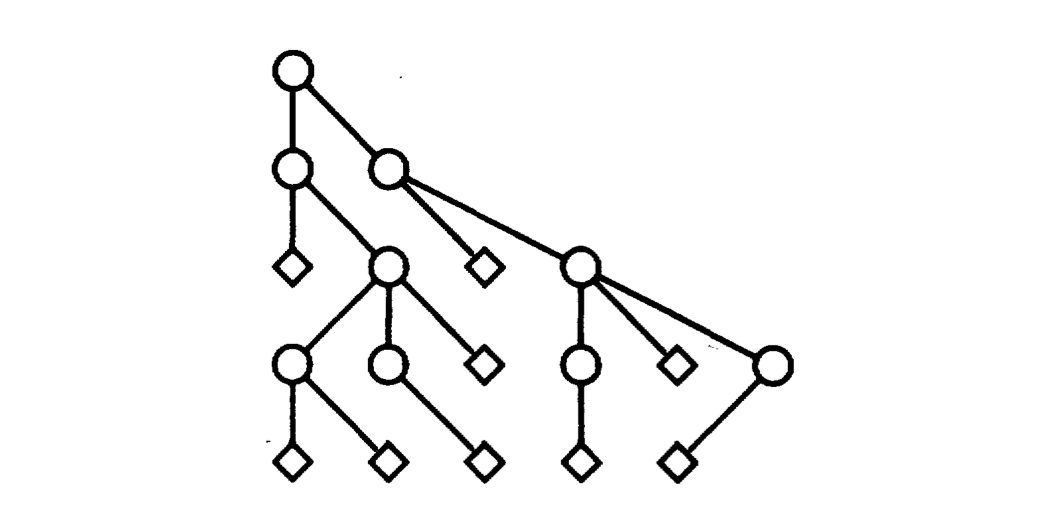
\includegraphics[scale=0.4]{arbreNaif.png}
    		\end{center}
    	\caption{Notre premier arbre modifié par l'\emph{Algorithme 1}. \cite{article79}}
      \label{fig:arbreNaif}
    \end{figure}
    \vfill

    \subsubsection{Binary Tree Drawings}

    L'algorithme que nous venons de voir est efficace, mais un problème se présente lorsque nous souhaitons faire apparaitre des labels sur les n\oe{}uds. Nous en venons maintenant à un algorithme qui nous permet de prendre en compte l'affichage de label sur notre graphe. Il a été conçu pour les arbres binaires (arbres avec deux fils maximum pour un n\oe{}ud).

    Les auteurs de l'article \cite{article79} font appel à une nouvelle propriété \emph{Esthétique 2} à respecter pour les ces arbres binaires: les fils de gauche doivent être placés à gauche de leur parent.

    \vfill
    \begin{figure}[h]
    		\begin{center}
    			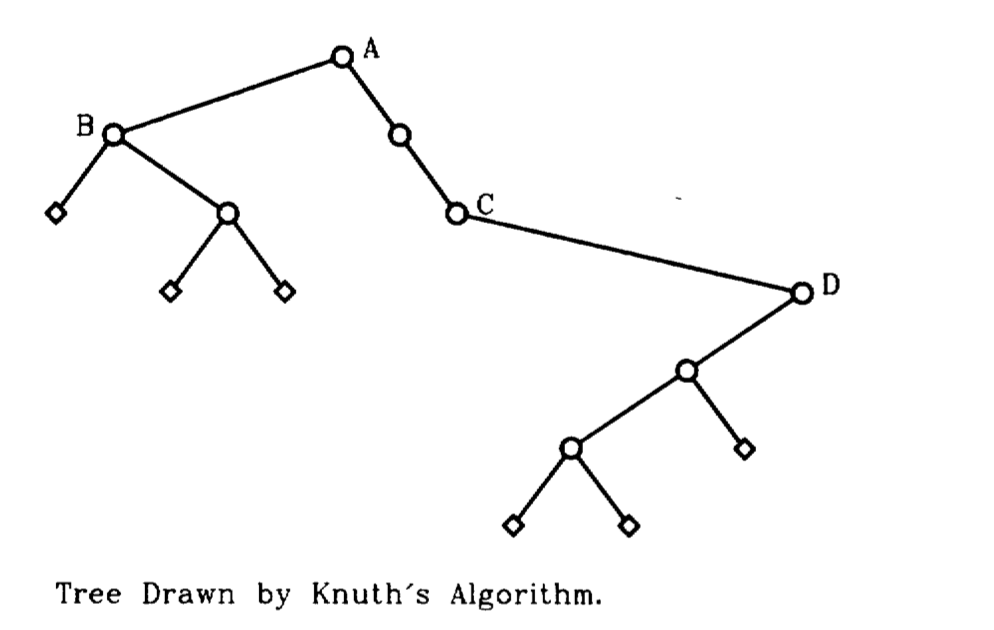
\includegraphics[scale=0.4]{arbreBinaire.png}
    		\end{center}
    	\caption{Arbre binaire dessiné par l'\emph{Algorithme de Knuth}. \cite{article79}}
      \label{fig:arbreBinaire}
    \end{figure}
    \vfill

    L'arbre binaire donné par ce nouvel algorithme respect bien les contraintes de l'\emph{Esthétique 1} ainsi que de l'\emph{Esthétique 2}, mais notre \emph{Limite physique 1} n'est pas respectée. L'algorithme fait en sorte que lorsqu’un n\oe{}ud occupe une colonne, nul autre n\oe{}ud ne peut occuper cette colonne. Nous obtenons donc une largeur proportionelle au nombre total de n\oe{}ud dans l'arbre.

    Il est alors nécessaire d'utiliser un algorithme différent pour que les conditions de l'\emph{Limite Physique} soient respectées.

    \subsubsection{Drawings Satisfying the Physical Limit}

    Nous avons vu que l'\emph{Algorithme 1} et l'\emph{Algorithme de Knuth} satisfaisaient chacun des contraintes \emph{Esthétique}. L'idée est ici de fusionner les deux algorithmes pour obtenir un algorithme qui respecte à la fois l'\emph{Esthétique 1}, l'\emph{Esthétique 2} et la \emph{Limite Physique}. L'\emph{Algorithme 3} qui résulte de cette fusion donne des meilleurs arbres que l'\emph{Algorithme 2}, mais ne respecte pas la \emph{Limite Physique} dans toutes les situations.

    \vfill
    \begin{figure}[h]
        \begin{center}
      		\begin{left}
      			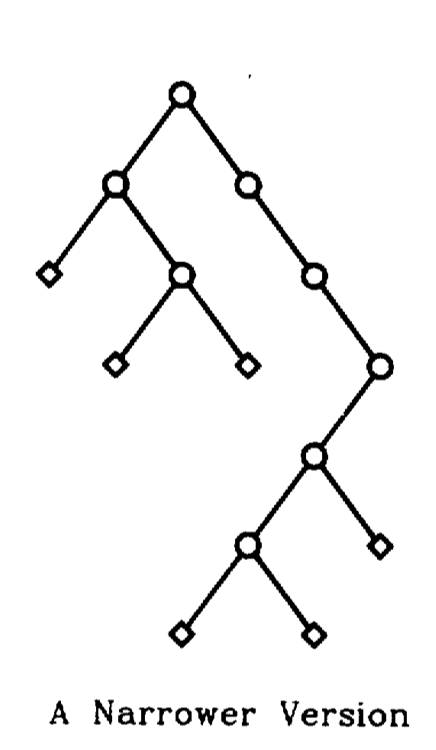
\includegraphics[scale=0.4]{arbreBinaireNarrow.png}
      		\end{left}
          \begin{right}
            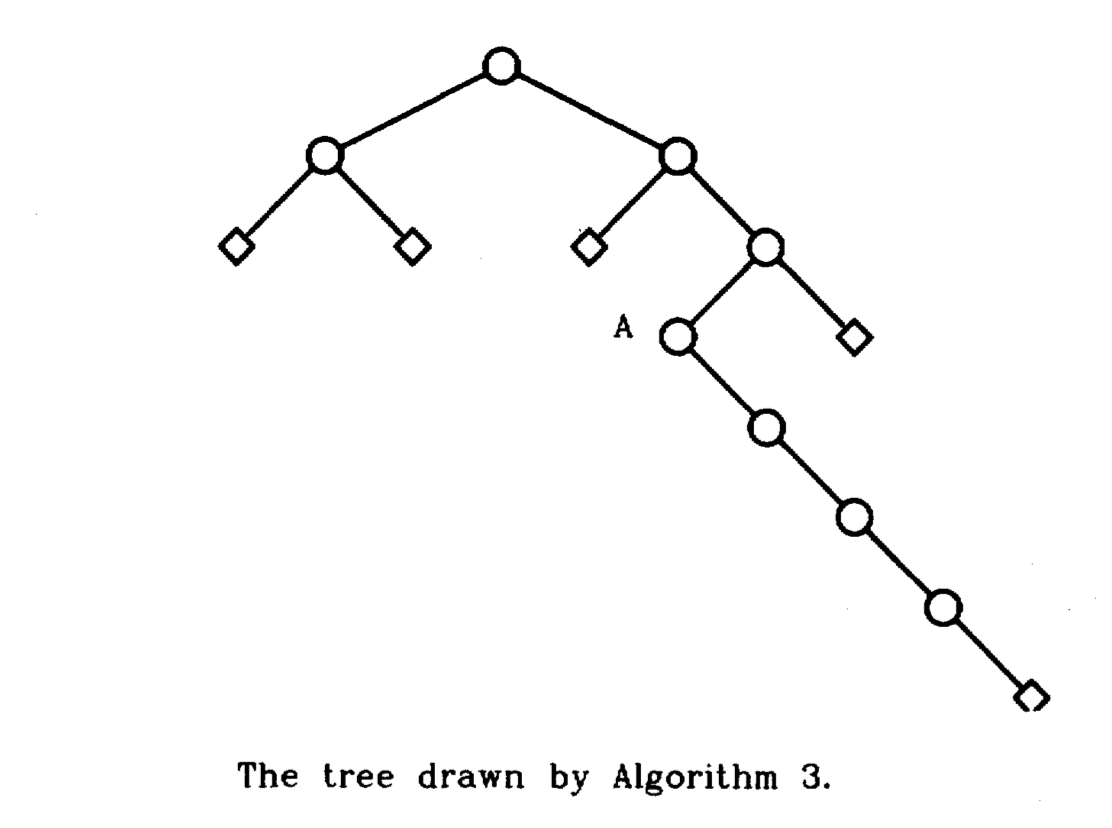
\includegraphics[scale=0.4]{arbre3.png}
          \end{right}
        \end{center}
    	\caption{À gauche l'arbre binaire vu précédement à la Figure \ref{fig:arbreBinaire}; à droite un autre arbre en sortie du même algorithme.  \cite{article79}}
      \label{fig:arbresAlgo3}
    \end{figure}
    \vfill

    \newpage
    L'arbre binaire que nous avons vu à la suite de l'\emph{algorithme de Knuth} est à présent optimal en largeur. Il restpect les contraintes de la \emph{Limite Physique}. Nous constatons que l'arbre qui est à droite, par contre, pourrait être plus optimisé. Il résulte de ce contre exemple que l'\emph{Algorithme 3} doit être modifié afin d'obtenir de meilleurs résultats.

    Face à ce problème, les auteurs de l'article \cite{article79} ont posé une nouvelle propriété \emph{Esthétique 3}: les parents doivent être centrés par rapport à leurs fils. Cela incluant leur fils directs, mais aussi les fils de leur fils.

    Le but étant qu'une fois l'\emph{Algorithme 3} modifié, notre nouvel algorithme respectera donc l'\emph{Esthétique 1}, \emph{Esthétique 2}, \emph{Esthétique 3} et la \emph{Limite Physique}.

    \vfill
    \begin{figure}[h]
        \begin{center}
      		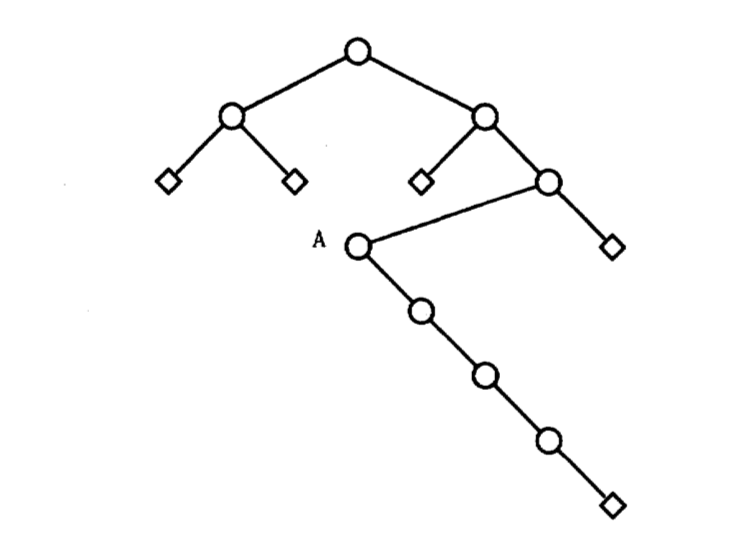
\includegraphics[scale=0.5]{arbre3Modifie.png}
        \end{center}
    	\caption{Arbre de droite de la Figure \ref{fig:arbresAlgo3} après l'utilisation de l'\emph{Algorithme 3 Modifié}. \cite{article79}}
      \label{fig:arbresAlgo3Modifie}
    \end{figure}
    \vfill

  \subsection{\emph{Tidier Drawings of Trees}}
  \subsection{\emph{A Node-Positioning Algorithm for General Trees}}
  \subsection{\emph{Improving Walker’s Algorithm to Run in Linear Time}}


\newpage
\section{Implémentation des algorithmes}

\newpage
\section{Étude empirique des algorithmes}

\newpage
\section{Conclusion}




\newpage
\medskip

\begin{thebibliography}{10}

\bibitem{article79}
C. Wetherell and A. Shannon. Tidy Drawings of Trees. \textit{IEEE transactions on Software Engineering} SE-5, 5 (septembre 1979) p514-520.

\bibitem{article81}
E. Reingold and J. Tilford. Tidier Drawings of Trees. \textit{IEEE Transactions on Software Engineering} SE-7, 2 (mars 1981) p223-228.

\bibitem{article90}
J. Walker II. A Node-Positioning Algorithm for General Trees. \textit{Software – Practice and Experience} SE-20, 2 (1990) p685–705.

\bibitem{article02}
C. Buchheim, M. Jünger and S. Leipert. Improving Walker’s Algorithm to Run in Linear Time. Technical Report zaik2002-431, ZAIK, Universität zu Köln, (2002) p344-352.

\end{thebibliography}

\end{document}
